\section{Theory}
In this section the theory used throughout the thesis work is presented. This includes a presentation of the original model architectures used, the loss functions which were used, the optimization algorithm the models were trained with, various regularization techniques used to avoid overfitting and how to interpret ROC curves.

\subsection{Deep neural networks}
Deep neural networks is a branch of machine learning characterized by having several layers between the input and the output. Deep neural networks do not require manual engineering as they are capable of automatic discovery of tendencies and patterns in the training data, without any prior knowledge of the data. Deep neural networks employ the idea that natural high-level signals very often are composed of lower level signals, and thus by composing many layers of neurons in succession forms a deep structure which is capable of learning features on multiple levels of abstraction \cite{lecun}.\\
Common for all deep neural networks is, they are composed of the same basic components: neurons, weights, biases and activation functions. Each layer holds a number of neurons where each has its own weights and bias associated with it. The neurons in one layer is connected to a subset or all of the neurons in the next layer, feeding the next layer in the network with inputs. A neuron, its weights and its bias constitutes a linear function, but for the network to adapt to complex tendencies in the data, a non-linear activation function is applied to the output of the neuron. Common activation functions are \textit{ReLu}, \textit{Softmax} and \textit{sigmoid}.\\
During training a loss function is formulated and an optimization strategy employed to tune the parameters of the model optimally. Common loss functions are \textit{mean squared error} and \textit{cross entropy} and common optimization strategies include \textit{stochastic gradient descent} and \textit{Adam}. The loss function is used to estimate how well the model predicted, and effectively measures how much the model needs to be corrected to perform optimally. The optimization strategy is how the model should be changed according to the measured loss.

\subsection{Convolutional neural networks}
One type of deep neural networks are convolutional neural networks which are primarily build from convolutions. This allows the networks to work on images as a convolutional layer learns the weights of its convolution kernels. Convolutional neural networks are most commonly used for segmentation or classification tasks which requires processing of images \cite{CNN}.

\subsubsection{U-Net}
\begin{figure}
	\centering
	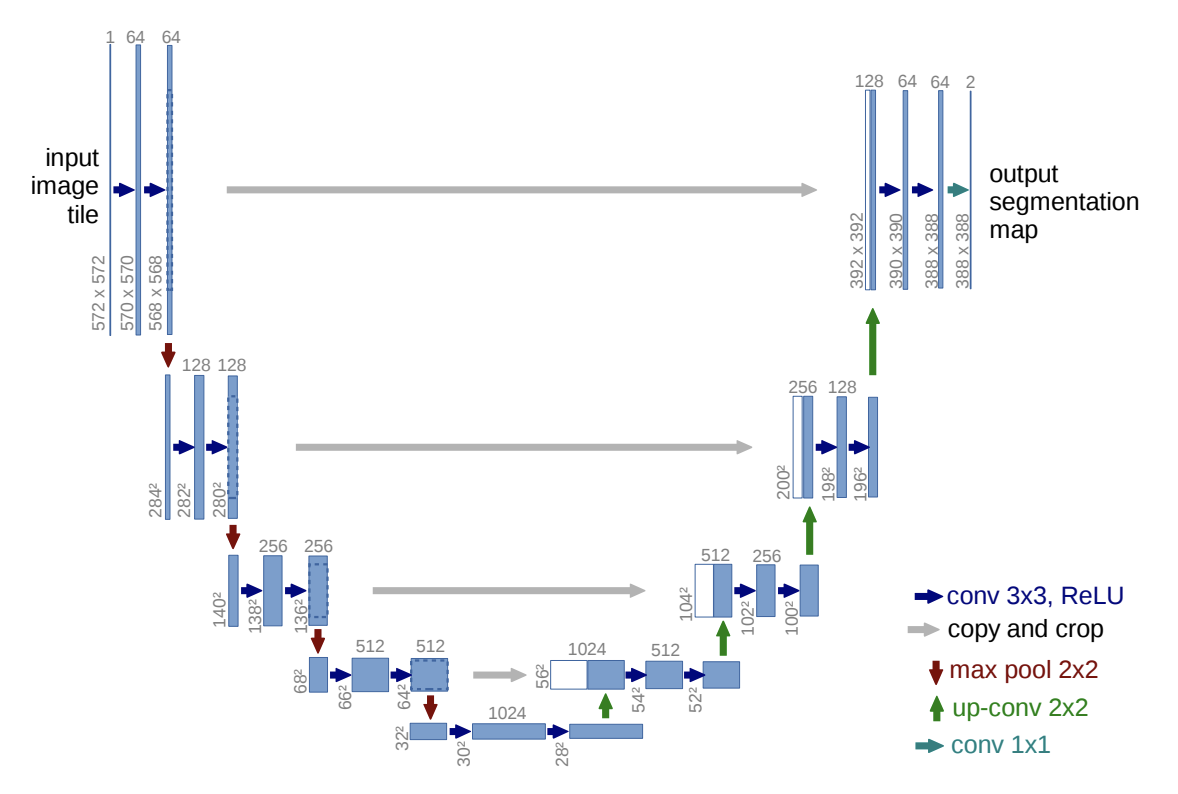
\includegraphics[width=\linewidth]{Materials/Theory/unet}
	\caption{U-Net model architecture for an input image of size 572x572. The number of feature channels is denoted on top of each blue box, and the image size is denoted on the side of the blue boxes. Illustration taken from \cite{unet}.}
	\label{unet}
\end{figure}

U-Net is a convolutional neural network architecture used for segmentation tasks. The network can be split in two parts, one which downscales the image, and one which upscales the image afterwards. The first part consists of three blocks where, in each, two convolutions are made before a max-pooling is performed. During the first convolution in a block the number of feature channels is doubled, and during the max-pooling the images are roughly halved in size. As the kernel sizes stays constant, and thus covers a larger portion of the images, this allows the U-Net to search for higher level features in the images. The second part also consists of three blocks with two convolutions each, however, now the number of feature channels are halved during the first convolution of the block, and the images are growing to twice its size after each upsampling is performed. After each upsampling a concatenation from the corresponding left part of the network is performed. These skip connections allows the model to recover lost spatial information and alleviates vanishing gradient issues. In the end, a 1x1 convolution is performed to map the output into the correct number of prediction classes. The output of U-Net is a segmentation of the input, and thus has the same size as its input image. An example of a U-Net can be seen in \autoref{unet} \cite{unet}.

\subsubsection{ResNet}
\begin{figure}[H]
	\centering
	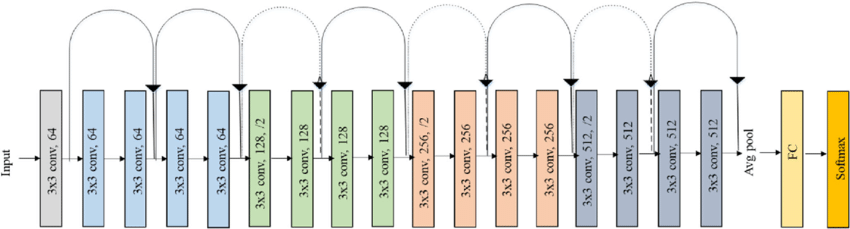
\includegraphics[width=\linewidth]{Materials/Theory/resnet}
	\caption{ResNet-18 model architecture consisting of a main path and identity residual connections. Illustration is taken from \cite{resnetModel}.}
	\label{resnet}
\end{figure}
ResNet is a convolutional neural network used for classification. The model comes in several sizes, but the core building blocks are the same across all variants. The ResNet consists of a main path and residual shortcuts. Looking at ResNet-18, the main path begins with a 7x7 convolution, a 3x3 max-pooling followed by four blocks, with four convolutions in each. At the end a global average-pooling is performed followed by a fully connected layer with a softmax. The residual shortcuts allows for some of the data to skip ahead in the network as an identity from previously in the network and is added to the output of a later convolution. These shortcuts can be directly used when the images are of same size, i.e. in the same block, but if a skip leads to a new block, padding with zeros or performing a 1x1 convolution is needed. The residual connections helps to alleviate vanishing gradients. The ResNet-18 architecture can be seen in \autoref{resnet}, and an illustration of how the residual connection works can be seen in \autoref{residualconnection} \cite{resnetPaper}.\\
As mentioned does ResNet come in several sizes where the number of blocks in the main path remain the same, but the number of convolutions in each varies from four in ResNet-18 to 108 in the block with most convolutions in ResNet-152. This makes a large difference in both depth of the network but also in the number of parameters the models contain. This makes it more difficult to train the larger versions, but it also makes the models more powerful as both the top-1 error and the top-5 error gets lower the more parameters the ResNet have \cite{resnet}.
\begin{figure}
	\centering
	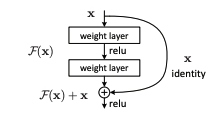
\includegraphics[width=0.5\linewidth]{Materials/Theory/ResidualConnection}
	\caption{Illustration of how the residual connections skip parts of the ResNet model. Illustration taken from \cite{resnetPaper}.}
	\label{residualconnection}
\end{figure}

\subsection{Loss functions}
\subsubsection{Cross entropy}
Cross entropy is a loss function which builds on the concept of entropy, and measures the difference between two probability distributions for a set of events, by computing the total entropy between the two probability distributions. The entropy is the number of bits requited to transmit a randomly selected event from a probability distribution. An asymmetric distribution will have low entropy due to the larger probability of certain events, whereas a more uniform distribution will have a larger entropy due to the events having closer to equal probability. The cross entropy is then the average number of bits required to encode an event from source distribution \textit{P} when using model distribution \textit{Q}. This can be seen as the number of additional bits needed to represent an event using an approximating distribution \textit{Q} rather than the original distribution \textit{P} \cite{crossentropy}.\\
In terms of a neural network and a multi class classification problem, only one class is considered correct, thus we can one-hot encode the target vector $\mathbf{y}$}, and use the result of a softmax activation as a prediction vector $\hat{\mathbf{y}}$. We can then compute the average cross entropy as:
\begin{equation*}
	CE = \frac{1}{N}\left(\sum_{i=1}^{N}\mathbf{y}_i\cdot log(\hat{\mathbf{y}}_i) \right)
\end{equation*}
For \textit{N} being the size of the training set.\\
Binary cross entropy is a special case of cross entropy where we only have two classes. This means the target $y$ is now either 1 or 0, and $\hat{y}$ is the model probability. The average binary cross entropy can be defined as:
\begin{equation*}
	BCE = \frac{1}{N}\sum_{i=1}^{N}\left[y_i\cdot log(\hat{y}_i)+(1-y_i)\cdot log(1-\hat{y}_i)\right]
\end{equation*}
For \textit{N} being the size of the training set. Cross entropy loss and binary cross entropy loss are commonly used for both segmentation and classification tasks.

\subsubsection{F1-score}
DICE coefficient or F1-score is a metric combining precision and recall. It can be defined as:
\begin{equation*}
	F1 = \frac{\text{TP}}{\text{TP}+\frac{1}{2}(\text{FP + FN})} = \frac{2\cdot\text{precision}\cdot\text{recall}}{\text{precision + recall}}
\end{equation*}
Where TP is the number of true positive predictions, FP is the number of false positive predictions and FN is the number of false negative predictions.\\
In terms of a binary segmentation task, it can also be formulated as two times the intersection between the target and predictions divided by the union of those:
\begin{equation*}
	F1 = \frac{2\cdot y \cap \hat{y}}{y\cup \hat{y}}
\end{equation*}
Where \textit{y} is the target and $\hat{y}$ is the predictions. This can intuitively be thought of as two times the number of correctly predicted pixels belonging to the segmentation class divided by the sum of the true number of pixels belonging to the segmentation class and the predicted number of pixels belonging to the segmentation class. Intuitively, if the models are accurate, the numerator will be half of the denominator, hence the multiplication by two. To convert the score to loss, we need to have $1 - \text{F1-score}$.\\
The advantage of evaluating model performance based on F1-score comes when the segmentation class is small compared to the total number of pixels in the image. Often it is easy to predict the background correctly, and thus, in tasks where large parts of the image is considered background, the accuracy of the model will inherently become large. However, this can be very misleading if very few, or any, predictions are correct in accordance to the segmentation class. Here the F1-score will be a much more accurate measure of model performance as it does not perform a pixel based accuracy measure, but measures the overlap of correct predictions belonging to the segmentation class.

\subsection{Optimization}
\subsubsection{Gradient descent}
Gradient descent is a first-order iterative optimization algorithm used to find a minimum of a differentiable function, and is widely used because of its simplicity and relative cheap computation cost. Gradient descent is based on the observation that if some function is differentiable in a neighbourhood, then its function value decreases fastest if one takes a small step in the direction of the negative gradient of the function. If small enough steps are taken in an iterative fashion, then it can be guaranteed that the algorithm converges to a local minima. When the function is convex, all local minima are global minima, and in this case the algorithm is guaranteed to converge to a global solution. More concretely, an initial guess, $\mathbf{x}_0$, for a local minima is made, and from here the position is iteratively updated as $\mathbf{x_{n+1} = \mathbf{x}_n - \gamma\nabla F(\mathbf{x_n})}$, where \textit{F} is the function, and $\gamma$ is the step size. Intuitively the algorithm can be thought of as having a ball rolling on a hill landscape where hill tops would correspond to local optima and valley bottoms would correspond to local minima. Placing the ball somewhere in this landscape will have it roll towards and stop near a valley bottom. As gradient descent only uses local information and simply takes a step in the steepest descent direction, it is prone to get stuck in local minima when used on pathological functions. If the step size is kept constant or decaying with a fixed rate, gradient descent can be slow at converging if the functions is very flat, and it can easily overshoot a minima if the function is very 'peaky' \cite{gradientdescent}. 1D and 2D examples of gradient descent can be seen in \autoref{gdIllustrations}.

\begin{figure}[H]
	\centering
	\begin{subfigure}{0.48\linewidth}
		\centering
		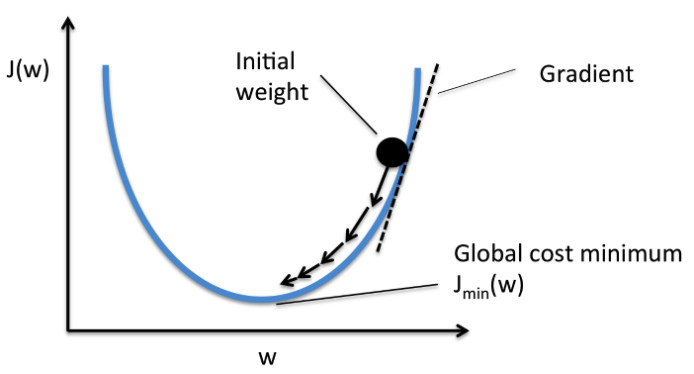
\includegraphics[width=\linewidth]{Materials/Theory/GD1D}
		\caption{Example of gradient descent in 1D, where the ball slowly rolls towards the global minimum.\newline}
	\end{subfigure}
	\hfill
	\begin{subfigure}{0.48\linewidth}
		\centering
		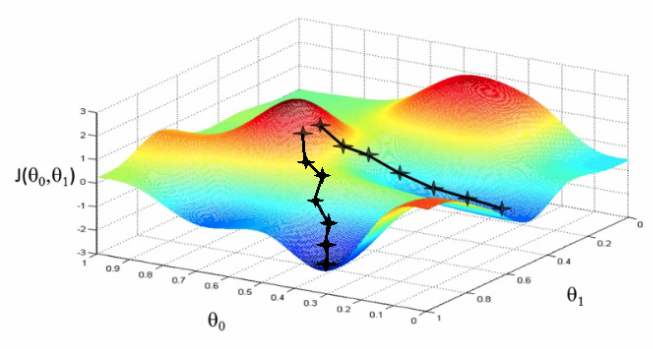
\includegraphics[width=\linewidth]{Materials/Theory/GD2D}
		\caption{Example of gradient descent in 2D, where two different initializations results in the algorithm terminating in two different minima.}
	\end{subfigure}
	\caption{Examples of gradient descent. Illustrations taken from \cite{GD1DIllustration}\cite{GD2DIllustration}.}
	\label{gdIllustrations}
\end{figure}

\subsubsection{Adam}
Adaptive moment estimation, Adam, is a stochastic gradient descent based optimization algorithm which is commonly used in all kinds of machine learning models. Adam makes three important improvements to traditional gradient descent. The first being each parameter in the model has its own adaptive learning rate. This means the step sizes for adjusting each parameter in the model will dynamically and independently be adjusted throughout training. The second improvement is, each learning rate can obtain momentum. This is important because as previously described, gradient descent can be slow at converging if the function is very flat, or it can overshoot a minima if the function is 'peaky'. With momentum, the prior gradient steps are taken into consideration when a new gradient step is performed, as a weighted average of gradients are computed. This results in less oscillation towards the minima, the option to get out of a local minima if large steps were taken but a flat spot is suddenly hit and the option to not immediately accelerate if small steps were taken but suddenly falling over a cliff. The last improvement is that, in general the learning rates should be larger at the beginning of training where we usually would be far away from a minima, and smaller towards the end where we need to be careful not to overshoot the minima \cite{adam}.

\subsection{Regularization}
Regularization is commonly used in machine learning to close the gap between performance on known and unknown data. As the end goal of machine learning is for the model to perform optimally on all data, including rare cases and unknown data, we want the model to generalize and learn a wide variety of features in the training data. However, if the model can simply look at a single common feature appearing in the training data, the model might weight this particular feature very heavily, and when it is then presented to unknown data where this feature is not present, the performance significantly drops. For this reason, regularization is employed to ensure the model learns a variety of features and is not reliant on observing one in particular. A wide range of regularization techniques exists, in the following four will be introduced. 

\subsubsection{Dropout}
Dropout is a regularization technique where a neuron with some probability \textit{p} is 'dropped' from the network. This means the neuron along its incoming and outgoing connections are temporarily removed from the network. At each epoch a new set of 'dropped' neurons are chosen according to the dropout probability \textit{p}, and the remaining neurons are thus forced to learn how to work with a randomly chosen set of other neurons. This drives each neuron towards creating useful features on its own, without relying on other neurons later correcting its mistakes. Dropout can be interpreted as adding noise to the neurons which forces the optimization to adopt random noise and thus generalize better. However, due to the added noise, the gradients computed during optimization are less accurate and the total number of training epochs needs to be increased \cite{dropout}.\\
Dropout is only employed during training as to gain the full potential of the network during testing. When we activate all neurons, the expected value of the next layer in the network increases by a factor of $\frac{1}{1-p}$ which leads to incorrect predictions. To avoid this we scale the weights by $\frac{1}{1-p}$  during training, or we can scale the weights by \textit{p} during testing \cite{dropout}. 

\subsubsection{Weight decay}
A simple solution to overfitting would be to decrease the number of parameters in our model. This would heavily limit its ability to overfit the training data, however, it would also heavily limit its ability to do predictions. More parameters can roughly be translated to more interactions between various parts of the network, and more interactions mean more non-linearities which helps us solve complex problems. However, the complexity of these interactions and of the model can get out of hand. To alleviate this, the squared sum of all weights in the model might be added as a term to our loss function to penalize complex models. This might, however, result in the loss getting so large, that the optimal weights are simply zero. For this reason, we introduce the weight decay as a small constant which is multiplied by the squared sum of the weights such that this regularization term is heavily reduced, and it is no longer optimal to have all weights being zero \cite{weightdecay}. 

\subsubsection{Normalization}
\begin{figure}[H]
	\begin{subfigure}{0.48\linewidth}
		\centering
		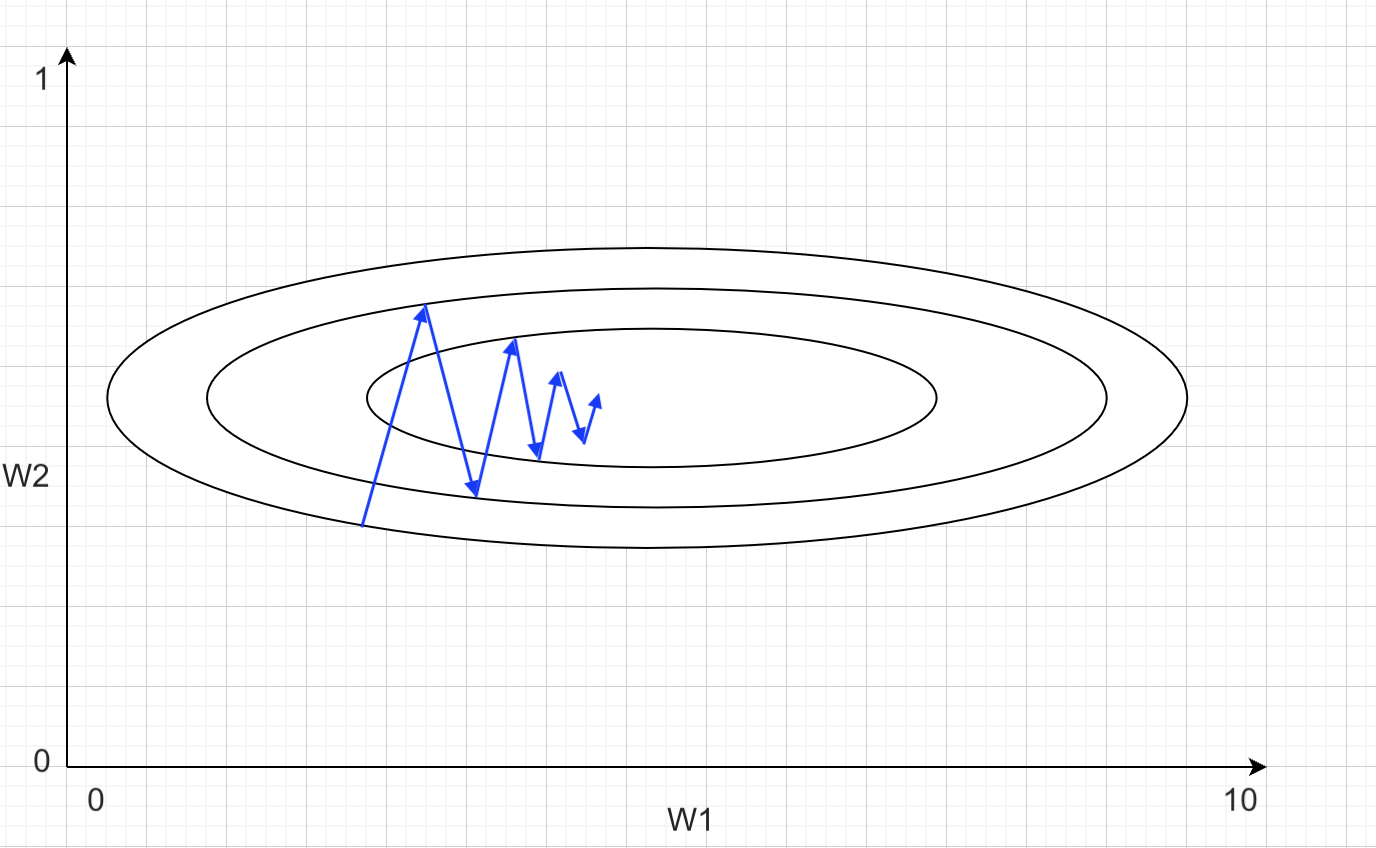
\includegraphics[width=\linewidth]{Materials/Theory/Normalization1}
		\caption{Non standardized data}
		\label{normalizationexamplea}
	\end{subfigure}
	\hfill
	\begin{subfigure}{0.48\linewidth}
		\centering
		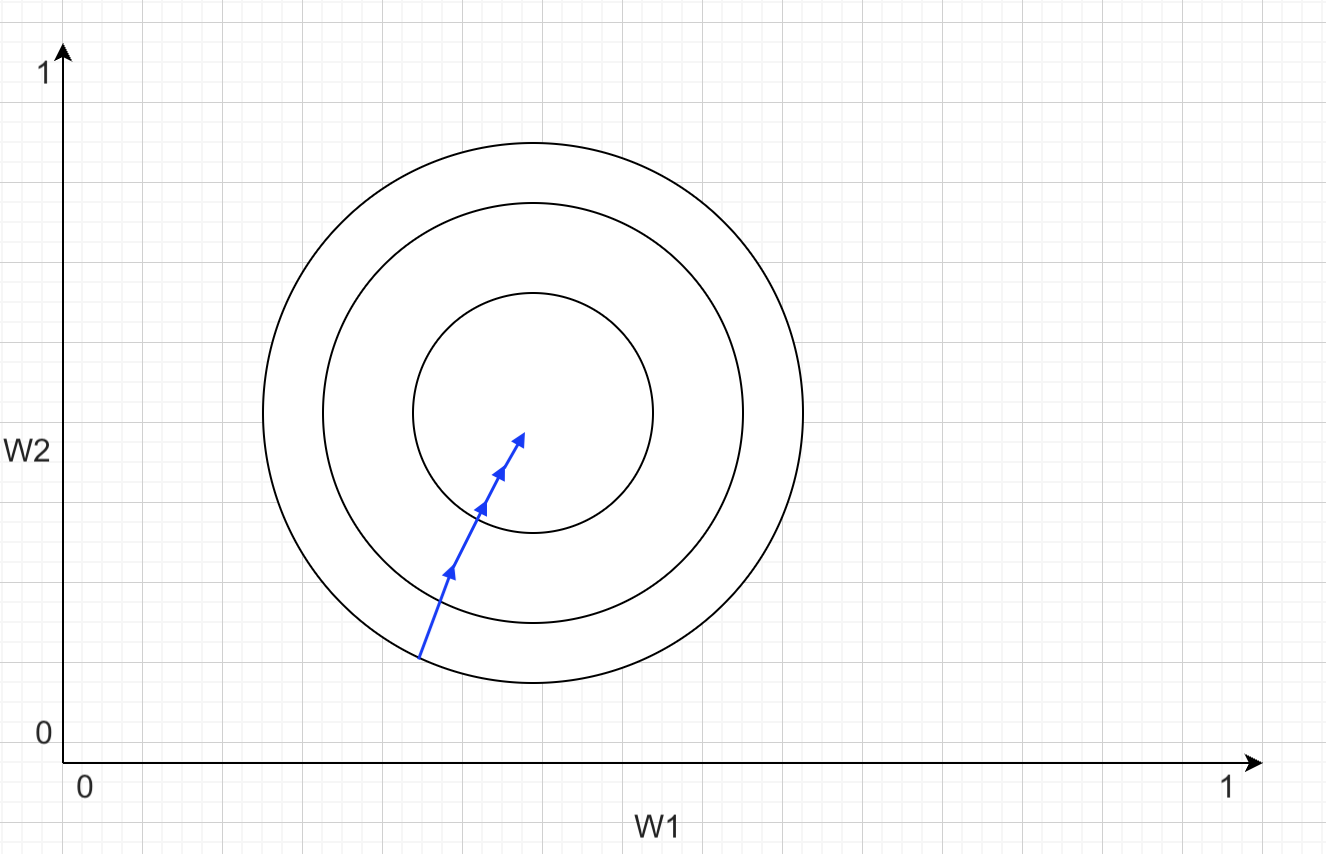
\includegraphics[width=\linewidth]{Materials/Theory/Normalization2}
		\caption{Standardized data}
		\label{normalizationexampleb}
	\end{subfigure}
	\caption{Examples of gradient descent optimization on non-standardized data and on standardized data. The blue line is the gradient steps taken during optimization. If the data is not standardized, the error surface becomes elongated, and the gradient steps points away from the minima, resulting in the gradient steps becoming 'zig-zaggy' and inefficient. If the data is standardized, the error surface becomes less elongated, and the gradient steps points more directly towards the minima, resulting in more efficient gradient steps.}
\end{figure}
Often deep neural networks trained with gradient based optimization algorithms suffer from slow learning when trained on data that is not standardized, i.e. does not have zero mean and unit variance \cite{normalization}. This should be seen as if the data is not standardized, the error surfaces gets elongated and as a result the gradient step might point away from the minimum. In \autoref{normalizationexamplea} we see a training example of not having standardized data. The blue line represent the gradient steps taken, which are perpendicular to the contour lines giving the steepest descent direction. Because the data is not standardized, learning becomes 'zig-zaggy'. If we however standardize the data, the error surface is less elongated and the steepest descent direction points more directly towards the minima, giving us the example in \autoref{normalizationexampleb}, where the gradient steps are much more efficient and learning is thus much faster \cite{errorsurface}.

Because of this, when working with images, \textit{intensity normalization} is often employed. This implies each colour channel is standardized. In a medical setting, where several different imaging machines may have been used to obtain the data it can also help to standardize the data, as each machine might have slightly different outputs on the same input.\\
It is not only during the beginning of training we can benefit from normalization. Because the neuron's weights change during training, it is likely the distribution of the data between layers in the network changes, which is referred to as an internal covariate shift \cite{batchnormalization}. Internal covariate shifts can be reduced by introducing normalization into the network in the form of normalization layers. One such layer is known as a \textit{batch normalization} layer. In batch normalization the mean and variance is computed over each mini batch for a given layer:
\begin{equation*}
	\mu = \frac{1}{m}\sum_{i=1}^{m}x_i,\quad \sigma^2 = \frac{1}{m}\sum_{i=1}^{m}(x_i - \mu)^2
\end{equation*}
For \textit{m} being the number of samples in the mini batch. This mean and variance is then used to standardize the input:
\begin{equation*}
	\hat{x}_i = \frac{x_i - \mu}{\sqrt{\sigma^2+\epsilon}}
\end{equation*}
Where $\epsilon$ is introduced for numerical stability. Learnable parameters $\gamma$ and $\beta$ are then introduced to scale and shift the standardized data again:
\begin{equation*}
	y_i = \gamma\hat{x}_i + \beta
\end{equation*}
This is done because standardizing the data might constraint what a layer in the network is able to represent. An example would be that normalizing the the inputs of a sigmoid would constrain them to the linear regime of the non-linearity \cite{batchnormalization}. Thus, simply setting $\gamma = \sqrt{\sigma^2}$ and $\beta = \mu$ allows us to recover the un-normalized data, if that is optimal \cite{errorsurface}\cite{batchnormalization}.
\subsection{ROC curve}
When training binary classifiers a common performance measure is to draw the receiver operating characteristics (ROC) curve. The curve is drawn by plotting the true positive rate against the false positive rate for several thresholds. The true positive rate is computed as $\frac{TP}{TP+FN}$ where \textit{TP} is the true positives, and \textit{FN} is the false negatives. The false positive rate is computed as $\frac{FP}{TN+FP}$ where \textit{FP} is the false positives and \textit{TN} is the true negatives. In a binary classification problem the class with a predicted probability of more than $0.5$, is usually the class one denotes as the class the model predicted. But the threshold of $0.5$ could arbitrarily be changed, and by changing it we can draw ROC curves \cite{ROC}. ROC curves can thus be read as a measure of how many more false positives we introduce if we wish to increase the number of true positives.\\
The evaluation of a ROC curve is usually done by measuring the area under the curve which is between 0 and 1 with a higher area under the curve being better. If we think of the true negatives and the true positives as two distributions, we achieve the best results when the two distributions do not overlap. In this case we get a perfect separability of the two cases, and we get an area under the curve of 1. If the two distributions begins to overlap, however, we begin to see false negative and false positive predictions, and we get a slightly lower area under the curve. In the worst case, the two distributions match and lies on top of each other, and there is no distinction between true positives and true negatives. Here we get an area under the curve of $0.5$. When the model predicts all class 1 samples as class 0, and vice versa, we see an area under the curve of $0$. These scenarios are illustrated in \autoref{ROC} \cite{ROC}.

\begin{figure}[H]
	\centering
	\begin{subfigure}{0.48\linewidth}
		\vspace{0.3cm}
		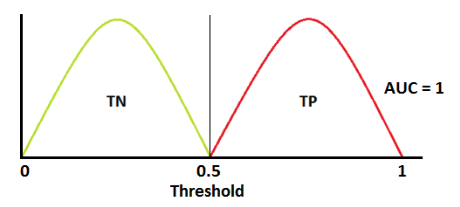
\includegraphics[width=\linewidth]{Materials/Theory/ROC1}
		\caption{When the two distributions do not overlap.}
	\end{subfigure}
	\hfill
	\begin{subfigure}{0.48\linewidth}
		\centering
		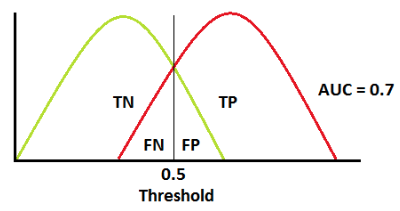
\includegraphics[width=\linewidth]{Materials/Theory/ROC2}
		\caption{When the two distributions slightly overlap.}
	\end{subfigure}
	\\
	\begin{subfigure}{0.48\linewidth}
		\centering
		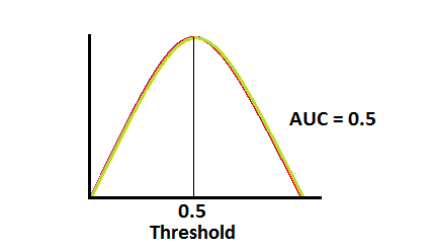
\includegraphics[width=\linewidth]{Materials/Theory/ROC3}
		\caption{When the two distributions are in indistinguishable.}
	\end{subfigure}
	\hfill
	\begin{subfigure}{0.48\linewidth}
		\vspace{0.8cm}
		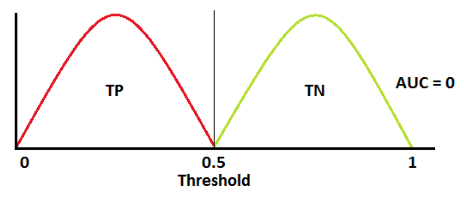
\includegraphics[width=\linewidth]{Materials/Theory/ROC4}
		\caption{When the model predicts all samples wrong.}
	\end{subfigure}
	\caption{Examples of how different area under the curve are achieved. Illustrations are from \cite{ROC}.}
	\label{ROC}
\end{figure}